\begin{frame}{VI in practice: The Criteo dataset}

As an example application of VB, consider a logistic regression with random
effects fit (generalized linear mixed model) to an internet advertising dataset
from Criteo Labs with $N=61895$ datapoints \citep[Section
5.3]{giordano2018covariances}.

We want to estimate:
%
\begin{align*}
%
\beta:{}&\quad\textrm{Regression parameters (5-dimensional)} \\
u:{}&\quad\textrm{Random effects (5000-dimensional)} \\
\mu:{}&\quad\textrm{Random effect mean (intercept)} \\
\tau:{}&\quad\textrm{Random effect precision (inverse variance)}.
%
\end{align*}
%
\pause

We use the following VB approximation:

\begin{center}
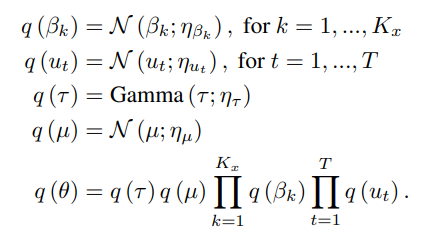
\includegraphics[width=0.45\textwidth]{static_images/Criteo_vb.png}
\end{center}

We will compare the joint MAP ($\approx$ MLE), MCMC, and the VB approximation.

\end{frame}



\begin{frame}{VI in practice: The Criteo dataset}

\begin{center}
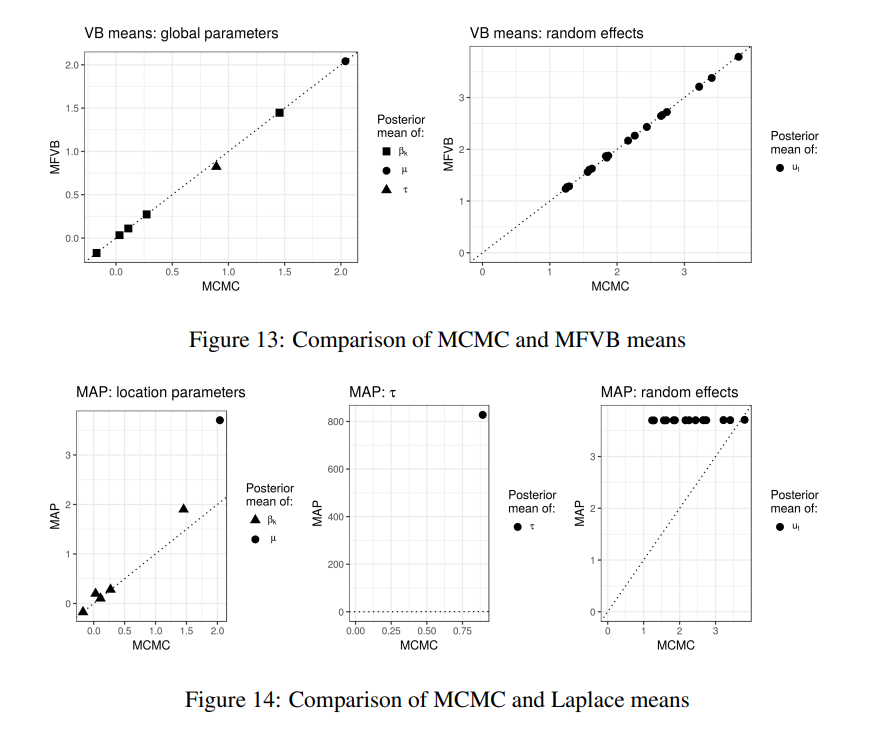
\includegraphics[width=0.9\textwidth]{static_images/Criteo_means.png}
\end{center}

\end{frame}



\begin{frame}{VI in practice: The Criteo dataset}

\begin{center}
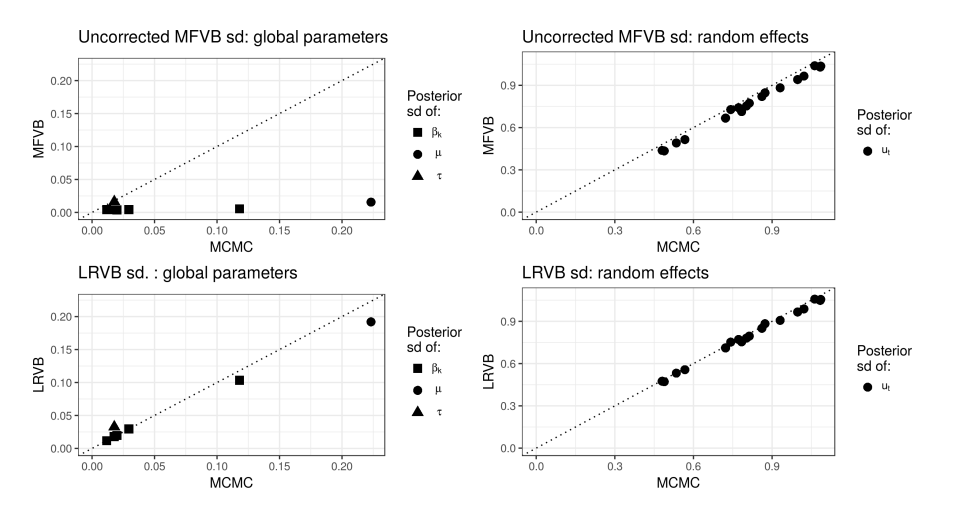
\includegraphics[width=0.9\textwidth]{static_images/Criteo_model_sds.png}
\end{center}


\begin{minipage}{0.6\textwidth}
%
Note that standard mean-field VB under-estimates posterior covariances.
We have a paper about alleviating this problem using
``linear response.''
\citep{giordano2018covariances}

\vspace{1em}
The Hessian was singular at the MAP, so the Laplace approximation
could not be computed.

%
\end{minipage}
%
\begin{minipage}{0.3\textwidth}
\begin{center}
    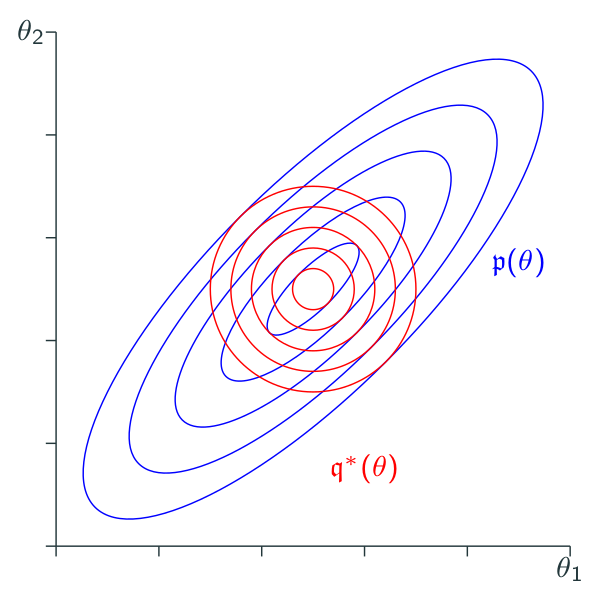
\includegraphics[height=1in]{static_images/mfvb_example.png}
\end{center}
\end{minipage}


\end{frame}


\begin{frame}{VI in practice: The Criteo dataset}

\begin{center}
VB is slower than the MAP, but much faster than MCMC.

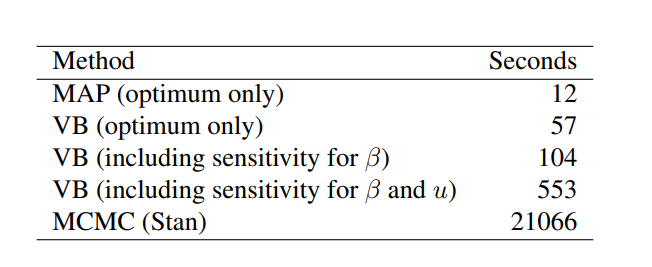
\includegraphics[width=0.6\textwidth]{static_images/Criteo_timing.png}
\end{center}

\end{frame}



\begin{frame}{VI in practice: Additional results}

\begin{center}
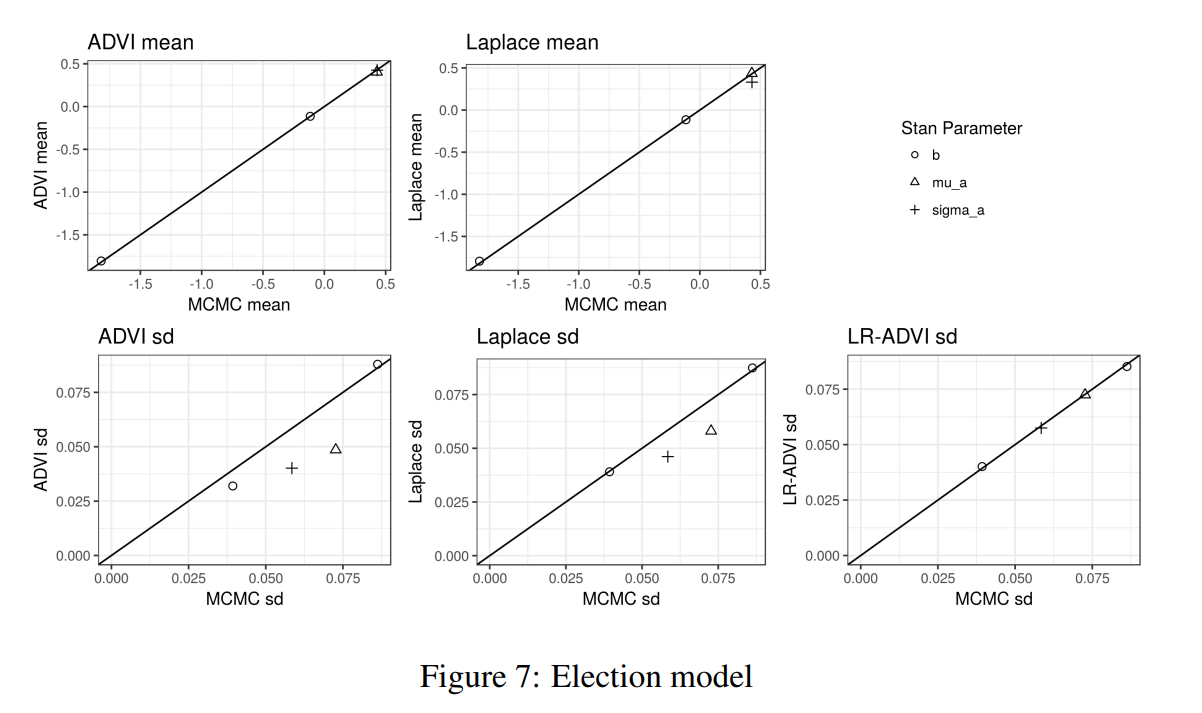
\includegraphics[width=0.9\textwidth]{static_images/Election_model.png}
\end{center}

\end{frame}



\begin{frame}{VI in practice: Additional results}

\begin{center}
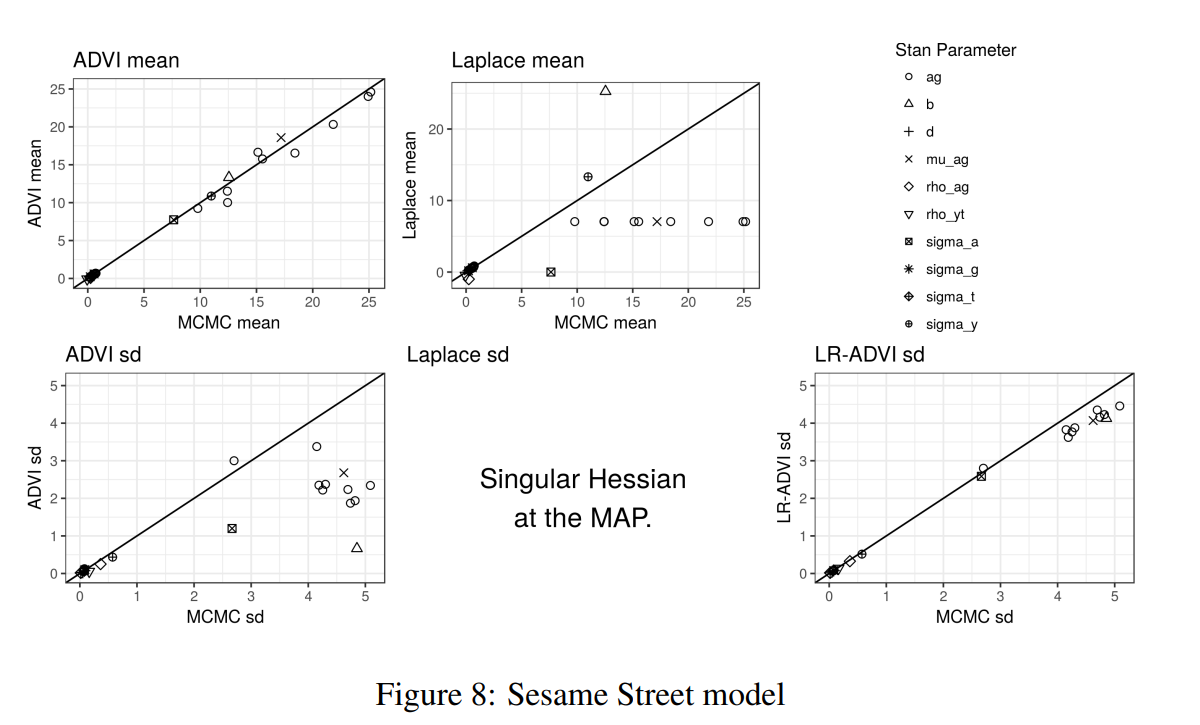
\includegraphics[width=0.9\textwidth]{static_images/Sesame_model.png}
\end{center}

\end{frame}



\begin{frame}{VI in practice: Additional results}

\begin{center}
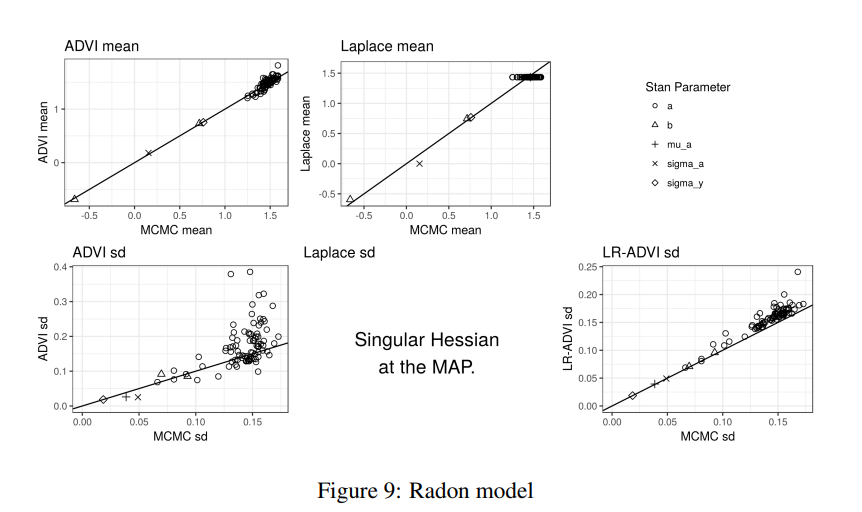
\includegraphics[width=0.9\textwidth]{static_images/Radon_model.png}
\end{center}

\end{frame}



\begin{frame}{VI in practice: Additional results}

\begin{center}
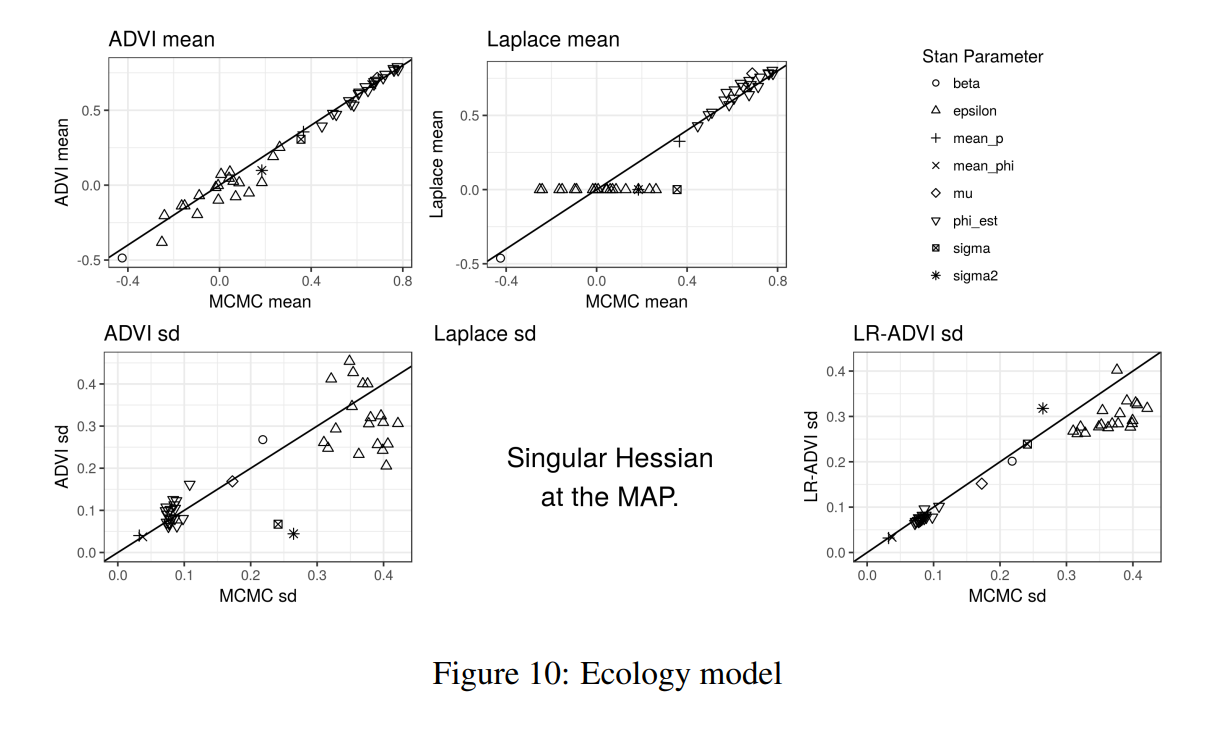
\includegraphics[width=0.9\textwidth]{static_images/CJS_model.png}
\end{center}

\end{frame}




\begin{frame}{VI in practice: Additional results}

\begin{center}
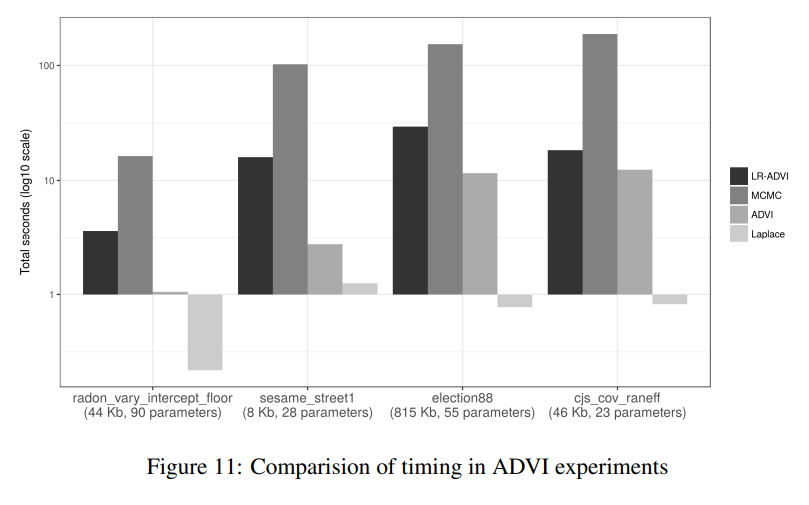
\includegraphics[width=0.9\textwidth]{static_images/advi_timing.png}
\end{center}

\end{frame}
